\section{Theorie}
\label{sec:Theorie}

\subsection{Schwingungsgleichungen für kapazitiv gekoppelte Schwingkreise}
Es werden im Folgenden zwei baugleiche elektrische Schwingkreise, mit jeweils den gleichen Induktivitäten L und Kapazitäten C betrachtet. Die Schwingkreise werden mit 
einem Kondensator mit variabler Kapazität $ C_k $ gekoppelt. (siehe Abbildung 1)
\begin{figure}
    \centering
    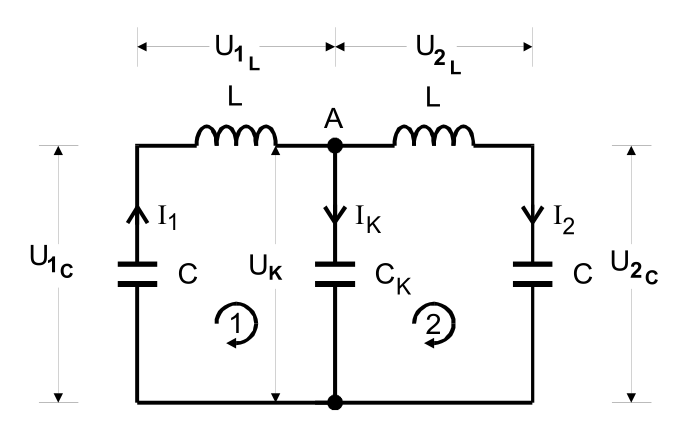
\includegraphics{Schaltung2.PNG}
    \caption{Prinzipschaltbild zweier gekoppelter Schwingkreise}
    \label{fig:DatenLangeSpule}
  \end{figure}
Mit Hilfe der Kirchhoffschen Knotenregel lässt sich für den Verzweigungspunkt A die Beziehung
\begin{equation}
    I_\text{k} = I_1 - I_2
    \label{eqn:Knotenregel}
  \end{equation}
  aufstellen.

Die Kirchhoffsche Maschenregel liefert zusätzlich jeweils für die beiden Leiterkreise 1 und 2 die Beziehung
\begin{equation}
    U_\text{C} + U_L + U_k = 0
    \label{eqn:Maschenregel}
  \end{equation}
Außerdem gilt
\begin{equation}
    U_\text{C} = \frac{1}{C} \int I \, \symup{d}t
  \end{equation}
  und
  \begin{equation}
    U_\text{L} = L \dot{I}
  \end{equation}
Setzt man diese Beziehung in (1) ein erhält man 
\begin{equation}
    \frac{1}{C} \int I_1 \, \symup{d}t + L \dot{I_1} + \frac{1}{C_k} \int I_1 - I_2 \, \symup{d}t = 0
\end{equation}
und
\begin{equation}
    \frac{1}{C} \int I_2 \, \symup{d}t + L \dot{I_2} - \frac{1}{C_k} \int I_1 - I_2 \, \symup{d}t = 0
\end{equation}
Wenn man diese Gleichungen nun ein mal nach der Zeit differenziert und anschließend addiert(3) und subtrahiert(4) erhält man
\begin{equation}
    L \frac{d^2}{dt^2}(I_1 + I_2) + \frac{1}{C}(I_1 +I_2) = 0
    \label{eqn:Drei}
\end{equation}
und
\begin{equation}
    L \frac{d^2}{dt^2}(I_1 - I_2) + ( \frac{1}{C} + \frac{2}{C_k} ) (I_1 - I_2) = 0
    \label{eqn:Vier}
\end{equation}
Damit hat man zwei unabhänig voneinader lösbare Differentialgleichungen, die als neue Variablen die Summe und Differenz der Ströme $ I_1 $ und $ I_2 $ haben.

Aus den Lösungen der Differentialgleichungen (3) und (4) ergeben sich die Frequenzen
\begin{equation}
    v^{+} = \frac{1}{ 2\symup{\pi} \sqrt{L C}}
    \label{eqn:Fuenf}
\end{equation}
und
\begin{equation}
    v^{-} = \frac{1}{ 2\symup{\pi} \sqrt{L (\frac{1}{C} + \frac{1}{C_k})^{-1}}}
    \label{eqn:Sechs}
\end{equation}

Betrachtet man nun zwei Spezialfälle des Systems der gekoppelten Oszillatoren, so werden die Bedeutungen der Schwingungen (5) und (6) deutlich.

Nimmt man an, dass die Oszillation in beiden Schwingkreisen mit gleicher Amplitude und in Phase beginnt, also $ I_1 = I_2 $ gilt, dann wird die Differenzschwingung $ v^{-} $ (6)
Null und beide Oszillatoren schwingen gleichphasig mit der Frequenz $ v^{+} $ (5), die der des Einzeloszillators entspricht. Da sich die Ströme $ I_1 $ und $ I_2 $ konsequent
aufheben, liegt hierbei zu keinem Zeitpunkt Spannung am Kondensator $ C_k $ an.

Im zweiten Spezialfall wird angenommen, dass die Oszillatoren wieder mit gleicher Amplitude, jedoch entgegengesetzter Phase ($ I_1 = -I_2 $) beginnen zu schwingen. In diesem Fall
wird die Summenschwingung $ v^{+} $ (5) Null und die beiden Oszillatoren schwingen gegenphasig mit der höheren Frequenz $ v^{-} $.

Diese beiden Spezialfälle und die zugehörigen Frequenzen bezeichnet man als Fundamentalschwingungen.
\\
Regt man das System der gekoppelten Oszillatoren so an, dass nur ein Oszillator zu Beginn eine von Null verschiedene Amplitude besitzt, so ergeben sich vollkommen andere Ergebnisse.

Addiert man die Loesungen der Differentialgleichungen (3) und (4) zusammen und betrachtet sie unter den gennanten Anfangsbedingungen $ I_1 = 0 $ und $ I_2 \neq 0 $ so erhält man
\begin{equation}
    I_1(t) = \frac{1}{2} I_{1_0} (\cos v^{+} t + \cos v^{-} t )
    \label{eqn:Sieben}
\end{equation}
und
\begin{equation}
    I_2(t) = \frac{1}{2} I_{1_0} (\cos v^{+} t - \cos v^{-} t )
    \label{eqn:Acht}
\end{equation}
Mit Hilfe von Additionstheoremen kann man (7) und (8) umschreiben zu
\begin{equation}
    I_1(t) = I_{1_0} \cos \frac{1}{2} (v^{+} + v^{-}) t \cos \frac{1}{2} (v^{+} - v^{-}) t
    \label{eqn:Neun}
\end{equation}
und
\begin{equation}
    I_2(t) = I_{1_0} \cos \frac{1}{2} (v^{+} + v^{-}) t \cos \frac{1}{2} (v^{+} - v^{-}) t
    \label{eqn:Zehn}
\end{equation}

An (9) und (10) kann man ablesen, dass das System nun mit einer Frequenz von $ \frac{1}{2} (v^{+} + v^{-}) $ oszilliert. Für diese Art von Oszillationen, die man Schwebungen nennt,
nimmt man an, dass sich die Frequenzen $ v^{+} $ und $ v^{-} $ nur gering voneinander unterscheiden. Demnach sind die Frequenz $ \frac{1}{2} (v^{+} + v^{-}) $ und
die Frequenz des Einzeloszillators $ v^{+} $ ungefähr gleich.

Ebenso kann man an (9) und (10) ablesen, dass die Amplitude mit der Frequenz $ v^{-} - v^{+} $ zwischen Null und $ I_{1_0} $ oszilliert. Diese Frequenz nannt man Schwebungsfrequenz.
\\
\subsection{Berechnung des Stromes in Abhängigkeit der Frequenz}
Regt man den in Abbildung 2 dargestellten Schwingkreis durch eine Sinusspannung zu einer erzwungenen Schwingung an,

ABBILDUNG 4 EINFÜGEN

ABBILDUNG 4 EINFÜGEN

ABBILDUNG 4 EINFÜGEN


so erhält man mit der Kirchhoffschen Maschenregel
\begin{equation}
    U = I_1 (z_C + z_L + z_{C_K} + z_R) - z_{C_K} I_2
    \label{eqn:Elf}
\end{equation}
und
\begin{equation}
    0 = I_2 (z_C + z_L + z_{C_K} + z_R) - z_{C_K} I_1
    \label{eqn:Zwoelf}
\end{equation}
\\
mit \begin{CenterStrip} 
        $z_C = -j \frac{1}{wC}$,$z_L = jwL$,   $z_{C_K} = -j \frac{1}{wC_K}$  und  $z_C = R$
    \end{CenterStrip}
\\

    Für $I_2$ folgt nach Elimination von $I_1$
\begin{equation}
    I_2 = U \frac{-j\frac{1}{wC_k}}{(jwL - j(\frac{1}{wc} + \frac{1}{wC_k})+R)^2 + \frac{1}{w^2 {C_k}^2}}
\end{equation}
\\
\begin{equation}
    \implies I_2 = U \frac{ -2wC_kRZ(w) + j(- \frac{1}{wC_k} + wC_kZ^2(w) - wR^2C_k) }{ 4w^2C_k^2R^2Z^2(w) + ( \frac{1}{wC_k} - wC_kZ^2(w) + wR^2C_k )^2 }
\end{equation} 
mit
\begin{equation}
    Z(w) \coloneq wL - \frac{1}{w} (\frac{1}{C} + \frac{1}{C_k})
\end{equation}
\\
Für den Betrag ergibt sich dann
\begin{equation}
    \lvert I_2\rvert = \lvert U\rvert \frac{1}{ 4w^2C_k^2R^2Z^2(w) + ( \frac{1}{wC_k} - wC_kZ^2(w) + wR^2C_k )^2 }
\end{equation}
\\
Bei den Fundamentalfrequenzen erreicht der Strom seine Maxima
\begin{equation}
    \lvert I(w^{+})\rvert = \frac{1}{ R\sqrt{4 + \frac{R^2C_k^2}{LC}}}
\end{equation}
und
\begin{equation}
    \lvert I(w^{-})\rvert = \frac{1}{ R\sqrt{4 + \frac{R^2C_k^2}{LC}(1+\frac{C}{C_k})}}
\end{equation}
\\
Diese Maxima können durch 
\begin{equation}
    \lvert I(w^{+})\rvert \approx \lvert I(w^{-})\rvert \approx \frac{1}{2R}
\end{equation}